\documentclass[12pt]{article}
\usepackage[utf8]{inputenc}
\usepackage{amsmath}
\usepackage{graphicx}
\usepackage{float}
\usepackage[margin=1in]{geometry}
\usepackage{lineno}
\setlength{\parindent}{2em}
\setlength{\parskip}{1em}
\renewcommand{\baselinestretch}{1.2}
\newcommand\dbyd[2]{\frac{\mathrm d{#1}}{\mathrm d{#2}}}
\newcommand{\R}{\mathcal{R}}
\title{Intentional infect susceptible with disease induced mortality rate}

\begin{document}
\linenumbers
\maketitle

\section{Introduction}

We also have to consider intentionally infect susceptible individuals with disease induced mortality rate being considered.

\section{System of differential equations}

Since we have to consider disease induced mortality rate, we need to adjust our model by adding extra terms representing mortality rate.

The following assumptions are used:

\begin{itemize}
\item Birth and natural death rate are the same.
\item The latent period is short enough to be ignored.
\item All susceptible individuals are equally likely to be infected, and all infected individuals are equally infectious.
\end{itemize}

\begin{equation}\label{1}
\begin{split}
\dbyd{S}{t}&=\mu- \beta S(V+I)-rS-\mu S \,,\\
\dbyd{V}{t}&=\beta SV+rS-\gamma V -\mu V\,,\\
\dbyd{I}{t}&=\beta SI-\gamma I -\mu I\,,\\
\dbyd{M}{t}&=0.01\gamma V+0.3\gamma I\,,\\
\dbyd{R}{t}&=0.99\gamma V+0.7\gamma I-\mu R\,,
\end{split}
\end{equation}

Where $\beta$ is transmission rate, $\gamma$ is recovery rate, $\mu$ is the \emph{per capita} rate of birth and death, $r$ is the rate of intensional infection on susceptible individuals.

For simplicity, we now convert the system into dimensionless form using dimensionless time coordinate,
\begin{equation}
\tau=(\gamma+\mu)t \,,
\end{equation}

As the result, we obtain,

\begin{subequations}\label{1}
\begin{align}
\dbyd{S}{\tau}&=\epsilon-\eta S-\R_0 S(V+I)-\epsilon S\,, \\
\dbyd{V}{\tau}&=\R_0 SV+\eta S-V\,,\\
\dbyd{I}{\tau}&=\R_0 SI-I\,,\\
\dbyd{M}{\tau}&=0.01(1-\epsilon) V+0.3(1-\epsilon) I\,,\\
\dbyd{R}{\tau}&=0.99(1-\epsilon) V+0.7(1-\epsilon) I-\epsilon R\,,
\end{align}
\end{subequations}

Where $\epsilon=\frac{\mu}{\gamma+\mu}$, $\R_0=\frac{\beta}{\gamma+\mu}$, $\eta=\frac{r}{\gamma+\mu}$

\section{Endemic Equilibrium}

To find endemic equilibrium, first we let equation (3c) equal to 0, we get: $I=0$ or $S=\frac{1}{\R_0}$. If $S=\frac{1}{\R_0}$, then by substituting into (3b), we get:
\begin{equation}
\dbyd{V}{\tau}=\eta S=\frac{\eta}{\R_0} = 0.
\end{equation}
Therefore, $\eta=0$ is the only possible solution, but again, this implies no intentional infection, hence, solution $S=\frac{1}{\R_0}$ is rejected.

Once again, $I=0$ is our solution. Then we use this result to substitute back into equation (3a) and (3b), we obtain,

\begin{subequations}
\begin{align}
\hat{S} &= \frac{1}{\R_0}-\frac{2\eta}{\R_0(-(\eta+\epsilon-\epsilon\R_0)+\sqrt{(\eta+\epsilon-\epsilon\R_0)^2+4\R_0\epsilon \eta}+2\eta)}\,,\\
\hat{V} &= \frac{-(\eta+\epsilon-\epsilon\R_0)+\sqrt{(\eta+\epsilon-\epsilon\R_0)^2+4\R_0\epsilon \eta}}{2\R_0}\,,\\
\hat{I} &= 0\,,
\end{align}
\end{subequations}

Additionally, the Jacobian matrix of this system is,
\begin{equation}
\mathcal{J} =
\begin{bmatrix}
    \ -\eta-\R_0 (V+I)-\epsilon       & -\R_0 S     &-\R_0 S\\
    \ \R_0 V+\eta       & \R_0 S-1    &0\\
    \ \R_0 I       &0     &\R_0 S-1\\
\end{bmatrix}\,.
\end{equation}

Eigenvalues of Jacobian are ,
\begin{subequations}
\begin{align}
\lambda_1&=-1+\R_0 S\\
\lambda_2&=\frac{-1-\eta-\epsilon+\R_0 S-\R_0 V-i\R_0-\sqrt{(-1-\eta-\epsilon+\R_0 S-\R_0 V-i\R_0)^2+4(-\eta-\epsilon-i\R_0+\epsilon\R_0 S-\R_0 V)}}{2}\\
\lambda_3&=\frac{-1-\eta-\epsilon+\R_0 S-\R_0 V-i\R_0+\sqrt{(-1-\eta-\epsilon+\R_0 S-\R_0 V-i\R_0)^2+4(-\eta-\epsilon-i\R_0+\epsilon\R_0 S-\R_0 V)}}{2}
\end{align}
\end{subequations}

To decide the sign of the real parts of eigenvalues, we use equation (5a) to acquire the following:
\begin{equation}
\hat{S} = \frac{1}{\R_0}-\frac{2\eta}{\R_0(-(\eta+\epsilon-\epsilon\R_0)+\sqrt{(\eta+\epsilon-\epsilon\R_0)^2+4\R_0\epsilon \eta}+2\eta)}\,,
\end{equation}
Thus,
\begin{equation}
\R_0\hat{S}=1-\frac{2\eta}{(-(\eta+\epsilon-\epsilon\R_0)+\sqrt{(\eta+\epsilon-\epsilon\R_0)^2+4\R_0\epsilon \eta}+2\eta)}\,,
\end{equation}
\begin{equation}
-1+\R_0 S=-\frac{2\eta}{(-(\eta+\epsilon-\epsilon\R_0)+\sqrt{(\eta+\epsilon-\epsilon\R_0)^2+4\R_0\epsilon \eta}+2\eta)}<0\,,
\end{equation}
Therefore,
\begin{subequations}
\begin{align}
\Re(\lambda_1) &=-1+\R_0 S<0\,,\\
\Re(\lambda_2) &=\Re(\lambda_3)=\frac{-1+\R_0 S-\eta-\epsilon-\R_0 V}{2}<0\,,
\end{align}
\end{subequations}
We are able to conclude that EE is stable.

\section{Disease Free Equilibrium}
In the case where there is no infected individuals inside a population, we can assume that both $V$ and $I$ are 0.

Substitute $V=0$ into equation (3b),
\begin{equation}
\dbyd{V}{\tau}=\eta S =0\,,
\end{equation}

It follows that $S=0$ since $\eta$ is a non-zero rate. Consequently, if we use $S=0$ and substitute into equation (3a), we have,
\begin{equation}
\dbyd{S}{\tau}=\epsilon=0\,,
\end{equation}

Which is not valid. Therefore, we do not have a DFE for this model as well.

\section{Disease induced mortality rate at Endemic Equilibrium}

By using equation (5a) through (5c), we can find the mortality rate at EE,
\begin{equation}
\dbyd{M}{\tau}=0.01(1-\epsilon)V=\frac{0.01(1-\epsilon)[-(\eta+\epsilon-\epsilon\R_0)+\sqrt{(\eta+\epsilon-\epsilon\R_0)^2+4\R_0\epsilon \eta}]}{2\R_0}\,,
\end{equation}

By plotting it, we obtain the following graph,
\begin{figure}[H]
  \centering
  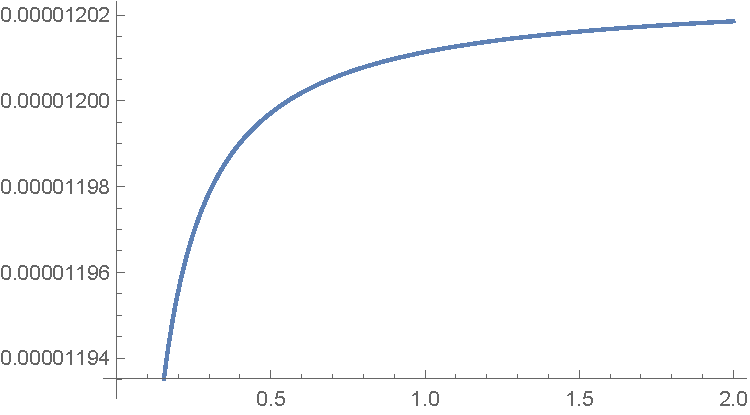
\includegraphics[width=1\textwidth]{Figures/M_at_EE.pdf}
  \caption{$\dbyd{M}{\tau}$ at EE as a function of $\eta$.}
\end{figure}

Interestingly, as $\eta$ increases, the disease induced mortality rate approaches a limit, which is,
\begin{equation}
\dbyd{M}{\tau}=0.0000120258\,.
\end{equation}

Though there exists a limit for $\dbyd{M}{\tau}$, but this occurs at an unreasonably high rate of intentional infection. However, this also means, at a low rate of intentional infection, the disease induced mortality rate at EE is controlled at a low rate as well.

\end{document}
